\documentclass[12pt]{article}
\usepackage{graphicx}

%
% Title.
\title{Experiment 1: Template}
% Author
\author{Aaron John Sabu, Roll Number 170070050}

% begin the document.
\begin{document}

% make a title page.
\maketitle

% section 1: overview.
\section{Overview of the experiment/assignment}

In two to three paragraphs, summarize 
\begin{itemize}
\item The purpose of the experiment/assignment.
\item What you did to perform the experiment/assignment.
\item Organization of your report and a summary of the
data you will be presenting.
\end{itemize}

You may refer to pre-existing documents by
citing them appropriately \cite{ref:Ramayana}.

For a more detailed introduction to the use of
LaTex to write documents, see \cite{ref:LatexTutorial}.

% section 2: setup/approach.
\section{Experiment setup or approach to the assignment}

Describe the experimental setup (or the approach you have used
to complete the assignment).

%
% You can include a figure in several formats. Here's a demo
% of how to include an eps file.
%
%  The figure is referred to by using the string "demofig",
%  latex will automatically number things correctly.
%
You can easily include a diagram/picture as shown in Figure \ref{fig:demofig}.
\begin{figure}
  % will center the figure.
  \centering
  % include graphics (can include eps, jpg, pdf ...)
  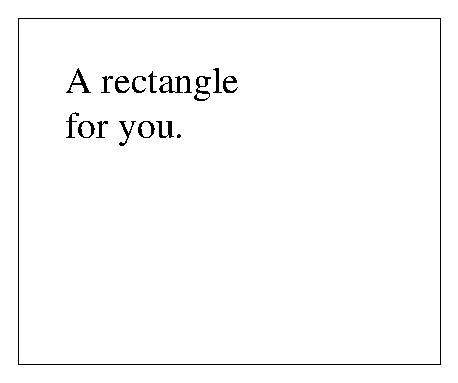
\includegraphics[scale=0.9]{figs/rectangle.eps}  % change scale factor to re-size the image.
  % give a caption.
  \caption{A rectangule.}
  % a label to refer to the figure
  \label{fig:demofig}
\end{figure}

\subsection{Include your design documentation and code if relevant}

You should give a brief description of whatever
designs you have constructed and a sketch of
the code you have written as part of the experiment/assignment.

To write code, you can use the verbatim environment.
(Note in verbatim mode, latex interprets your
text like a type-writer and does not do any formatting.  
Use spaces carefully to line things up).  There are other
latex environments such as {\em algorithm} which can 
be used to describe algorithms.
\begin{verbatim}
entity foo is
  -- ports.
  port (a: in bit; b: out bit);
end entity foo;
\end{verbatim}


\section{Observations}

You must summarize your observations, either in words, using
figures and/or tables.
%
% Tables.
%
You can easily include tables, such as the one shown in  Table \ref{table:demotable}.
\begin{table}
\centering  % table will be centered.
\begin{tabular}{|c | c c|} % 3 columns, with text centered in each column, 
			 %  the | specifies that there will be a line separating the
			 %  adjacent columns.
\hline  % horizontal line spanning the columns.
Item & W & H \\  % table entry 1, separated by &, ended by \\
\hline  % horizontal line spanning the columns.
A    & 2 & 3 \\  % table entry 2, separated by &, ended by \\
B    & 3 & 4 \\  % ...
C    & 4 & 5 \\  % ...
D    & 5 & 6 \\  % ...
\hline	% horizontal line.
\end{tabular}
\caption{Illustrative table}
\label{table:demotable}
\end{table}


%
% include a bibliography to give references to 
% material you have used.
% 
\begin{thebibliography}{99}
\bibitem{ref:Bible}
The Holy Spirit, The Holy Bible, over many centuries
%
% etc..
%
\bibitem{ref:LatexTutorial}
{\em https://www.latex-tutorial.com/tutorials/beginners/how-to-use-latex/}

\end{thebibliography}

\end{document}
